\documentclass{scrartcl}

\usepackage[utf8]{inputenc}
\usepackage[T1]{fontenc}
\usepackage{lmodern}
\usepackage[english]{babel}
\usepackage{amsmath}
\usepackage{graphicx}
\usepackage{caption}	
\usepackage{subcaption}	 
\usepackage{hyperref}
\usepackage[parfill]{parskip}
\usepackage{hhline}
\usepackage{subcaption}

\title{Neuroprosthetics - Exercise 5}
\author{Alexander Koenig}
\date{21. December 2019}

\begin{document}
\maketitle

\section{Create a Multi-Compartment Model}

The code from the previous programming exercise was altered to model the behavior of a sequence of cells and not just an individual cell. The cable equation and the resulting system of differential equations are solved numerically with the implicit Euler scheme. This results in the following linear system. To calculate the membrane potential in each cell for the next time step the system must be solved for $\vec{x}$. 

\begin{equation}
\underbrace{\left(\mathbf{I}-\frac{\Delta t}{C_{m} R_{a}} \mathbf{C}\right)}_{\mathbf{A}} \cdot \underbrace{\vec{V}_{m}(t+\Delta t)}_{\vec{x}}=\underbrace{\vec{V}_{m}(t)+\frac{\Delta t}{C_{m}}\left(-\vec{I}_{HH}(t+\Delta t)+\vec{I}_{s t i m}(t+\Delta t)\right)}_{\vec{b}}
\end{equation}
\begin{equation}
\mathbf{A} \cdot \vec{x}=\vec{b}
\end{equation}

100 ms long simulations are run at a temperature of 6.3$^\circ$C and with a time step of 25 $\mu$s. The stimulation currents are rectangular 5ms long pulses with an amplitude of 10 $\mu$A. Figures \ref{fig:1} and \ref{fig:2} show the formation and propagation of an action potential along the axon for two different cases. In the first case (figure \ref{fig:1}) a pulse stimulates the first compartment only, whereas in the second case the axon is stimulated simultaneously at compartment 20 and 80.

It is evident from both plots that the action potential propagates linearly. This is because the underlying model is a linear system of equations. In figure \ref{fig:2} both action potentials approach each other and destructively interfere at approximately 55 ms. Therefore in figure \ref{fig:2} no signal propagates further than approximately 60ms. This is because the neighboring compartments of the compartment in which the action potentials meet are still in their absolute refractory period. 

The three phases (depolarization, repolarization, hyperpolarization) of the action potential can be seen in the plots. The blue area describes the membrane at resting potential ($V_{rest} = 0$). Once the cell depolarizes the membrane potential spikes (red color). Immediately afterward the cell repolarizes (green color) and enters the longer hyperpolarization phase, which can be seen as a darker fade of blue after the action potential.

\begin{figure}
	\centering
	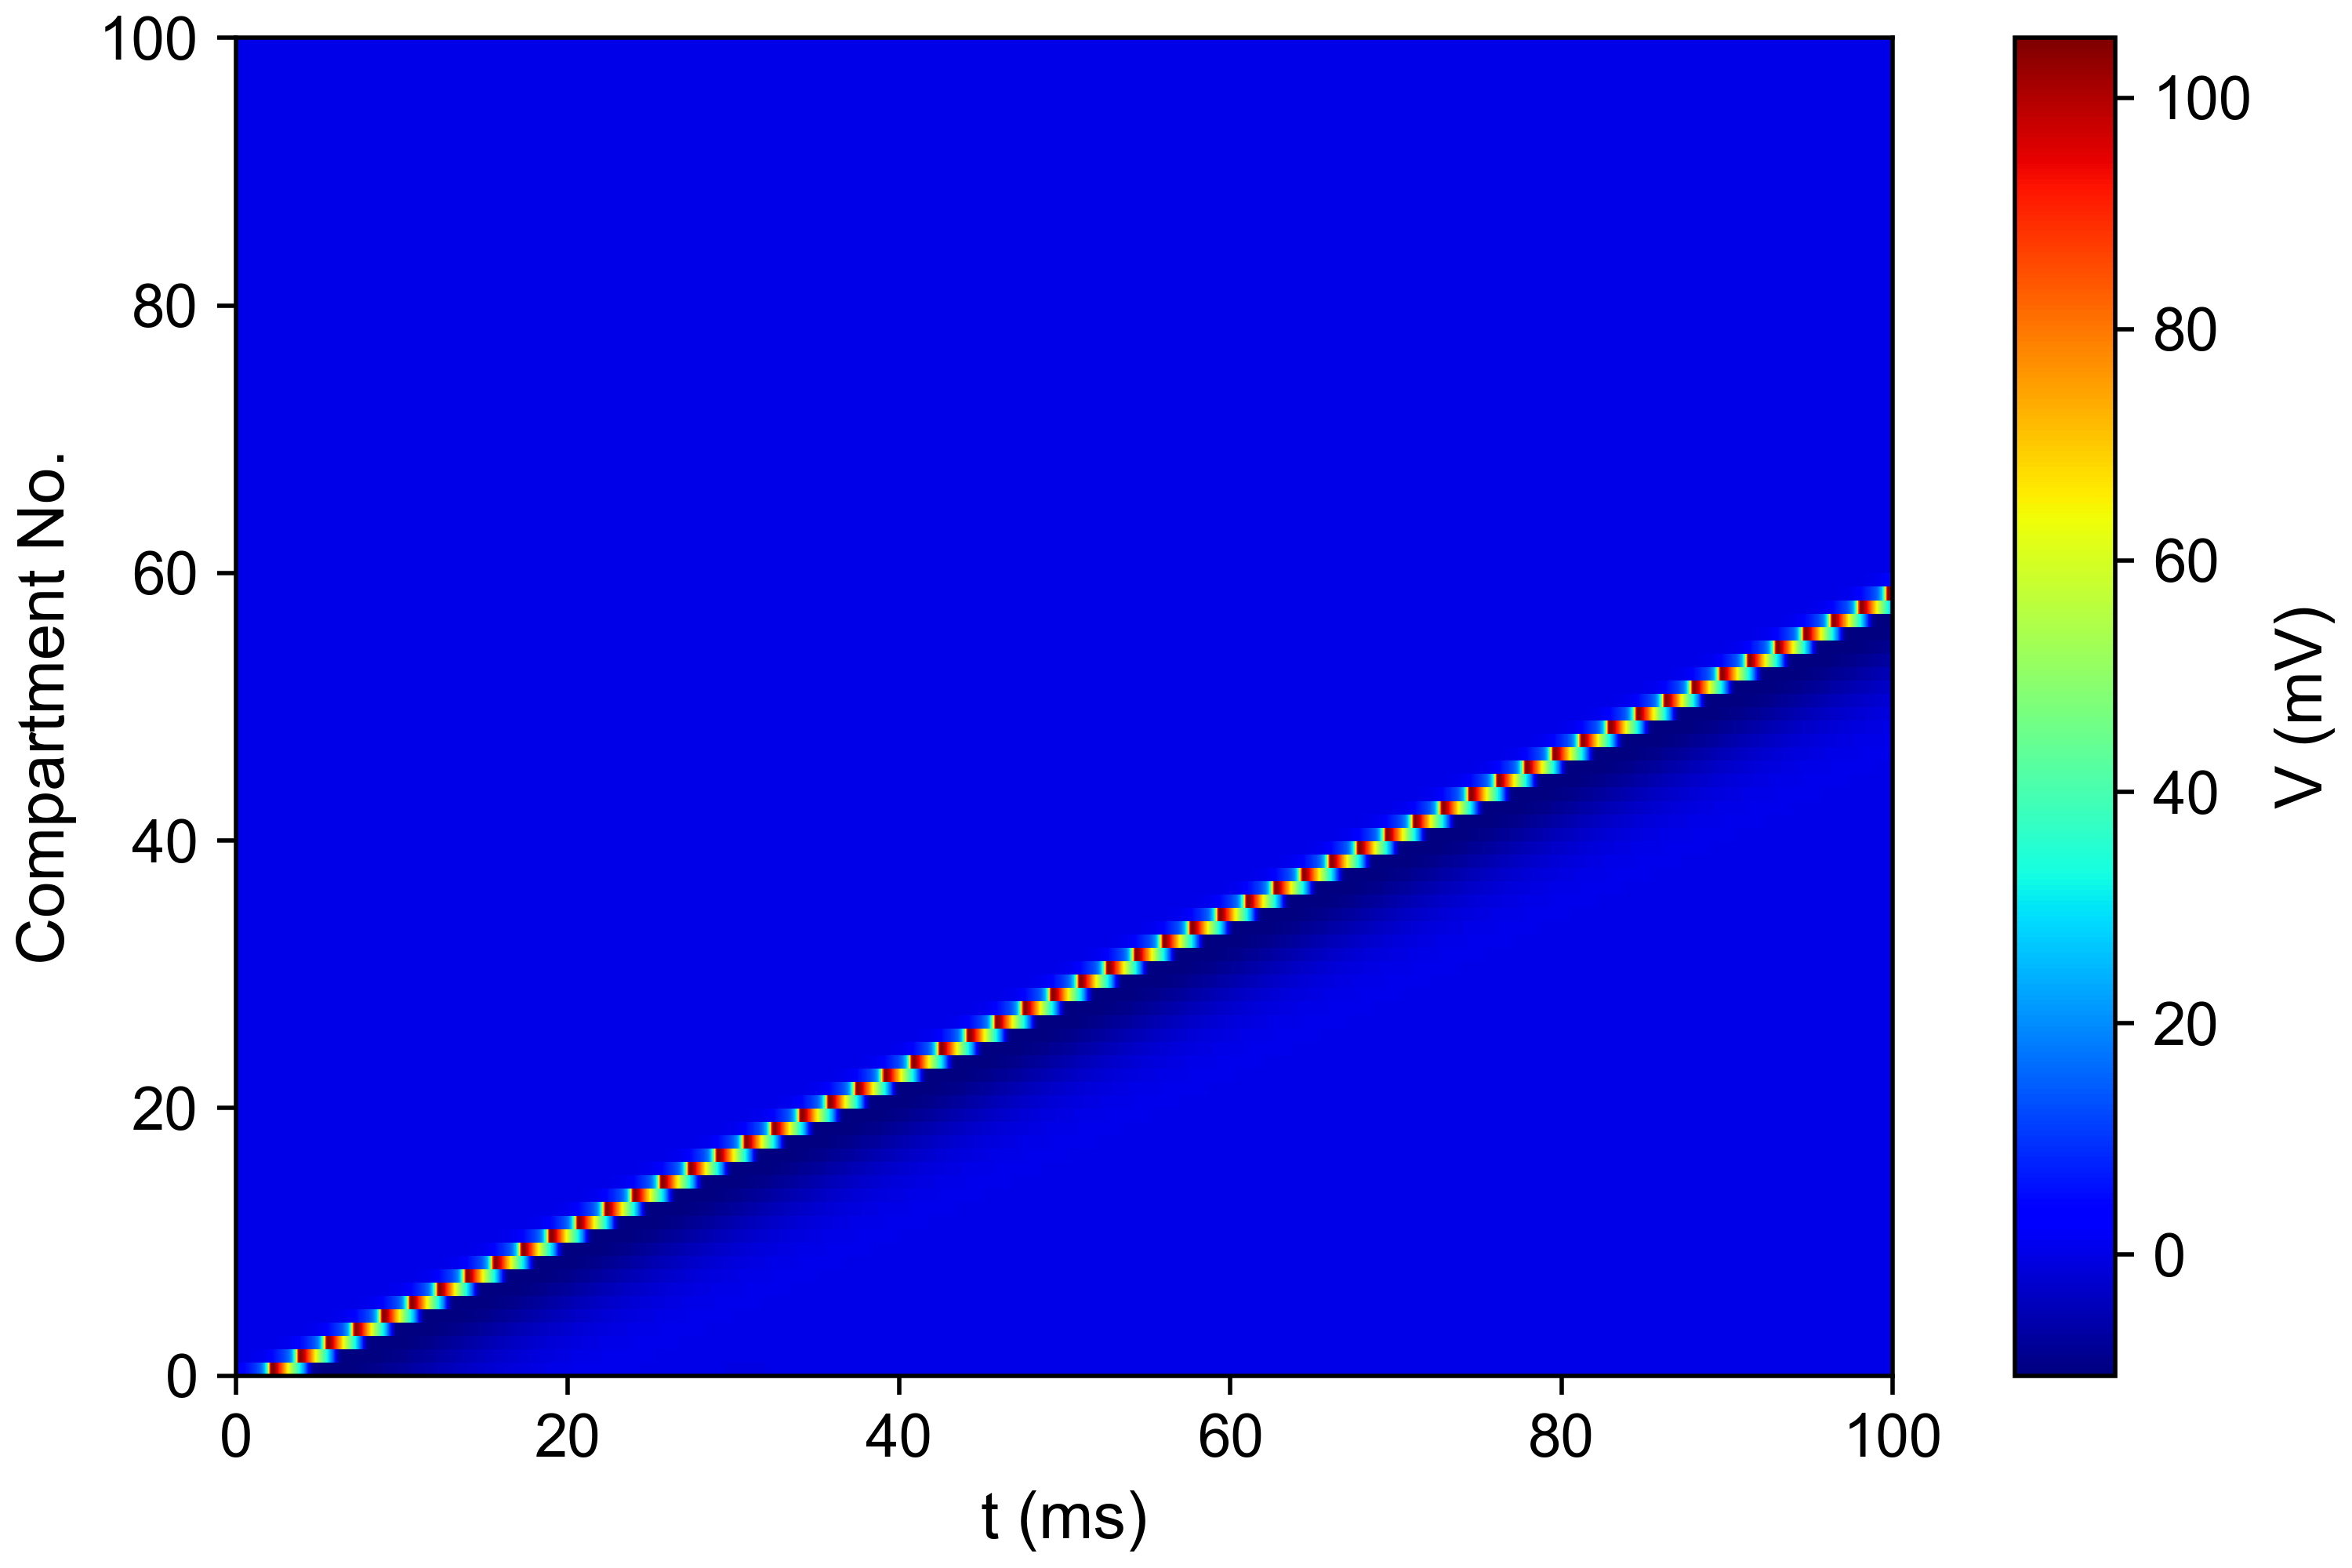
\includegraphics[width=0.9\textwidth]{figures/potential_case1.png}
	\caption{Potential for first case}
	\label{fig:1}
\end{figure}
\begin{figure}
	\centering
	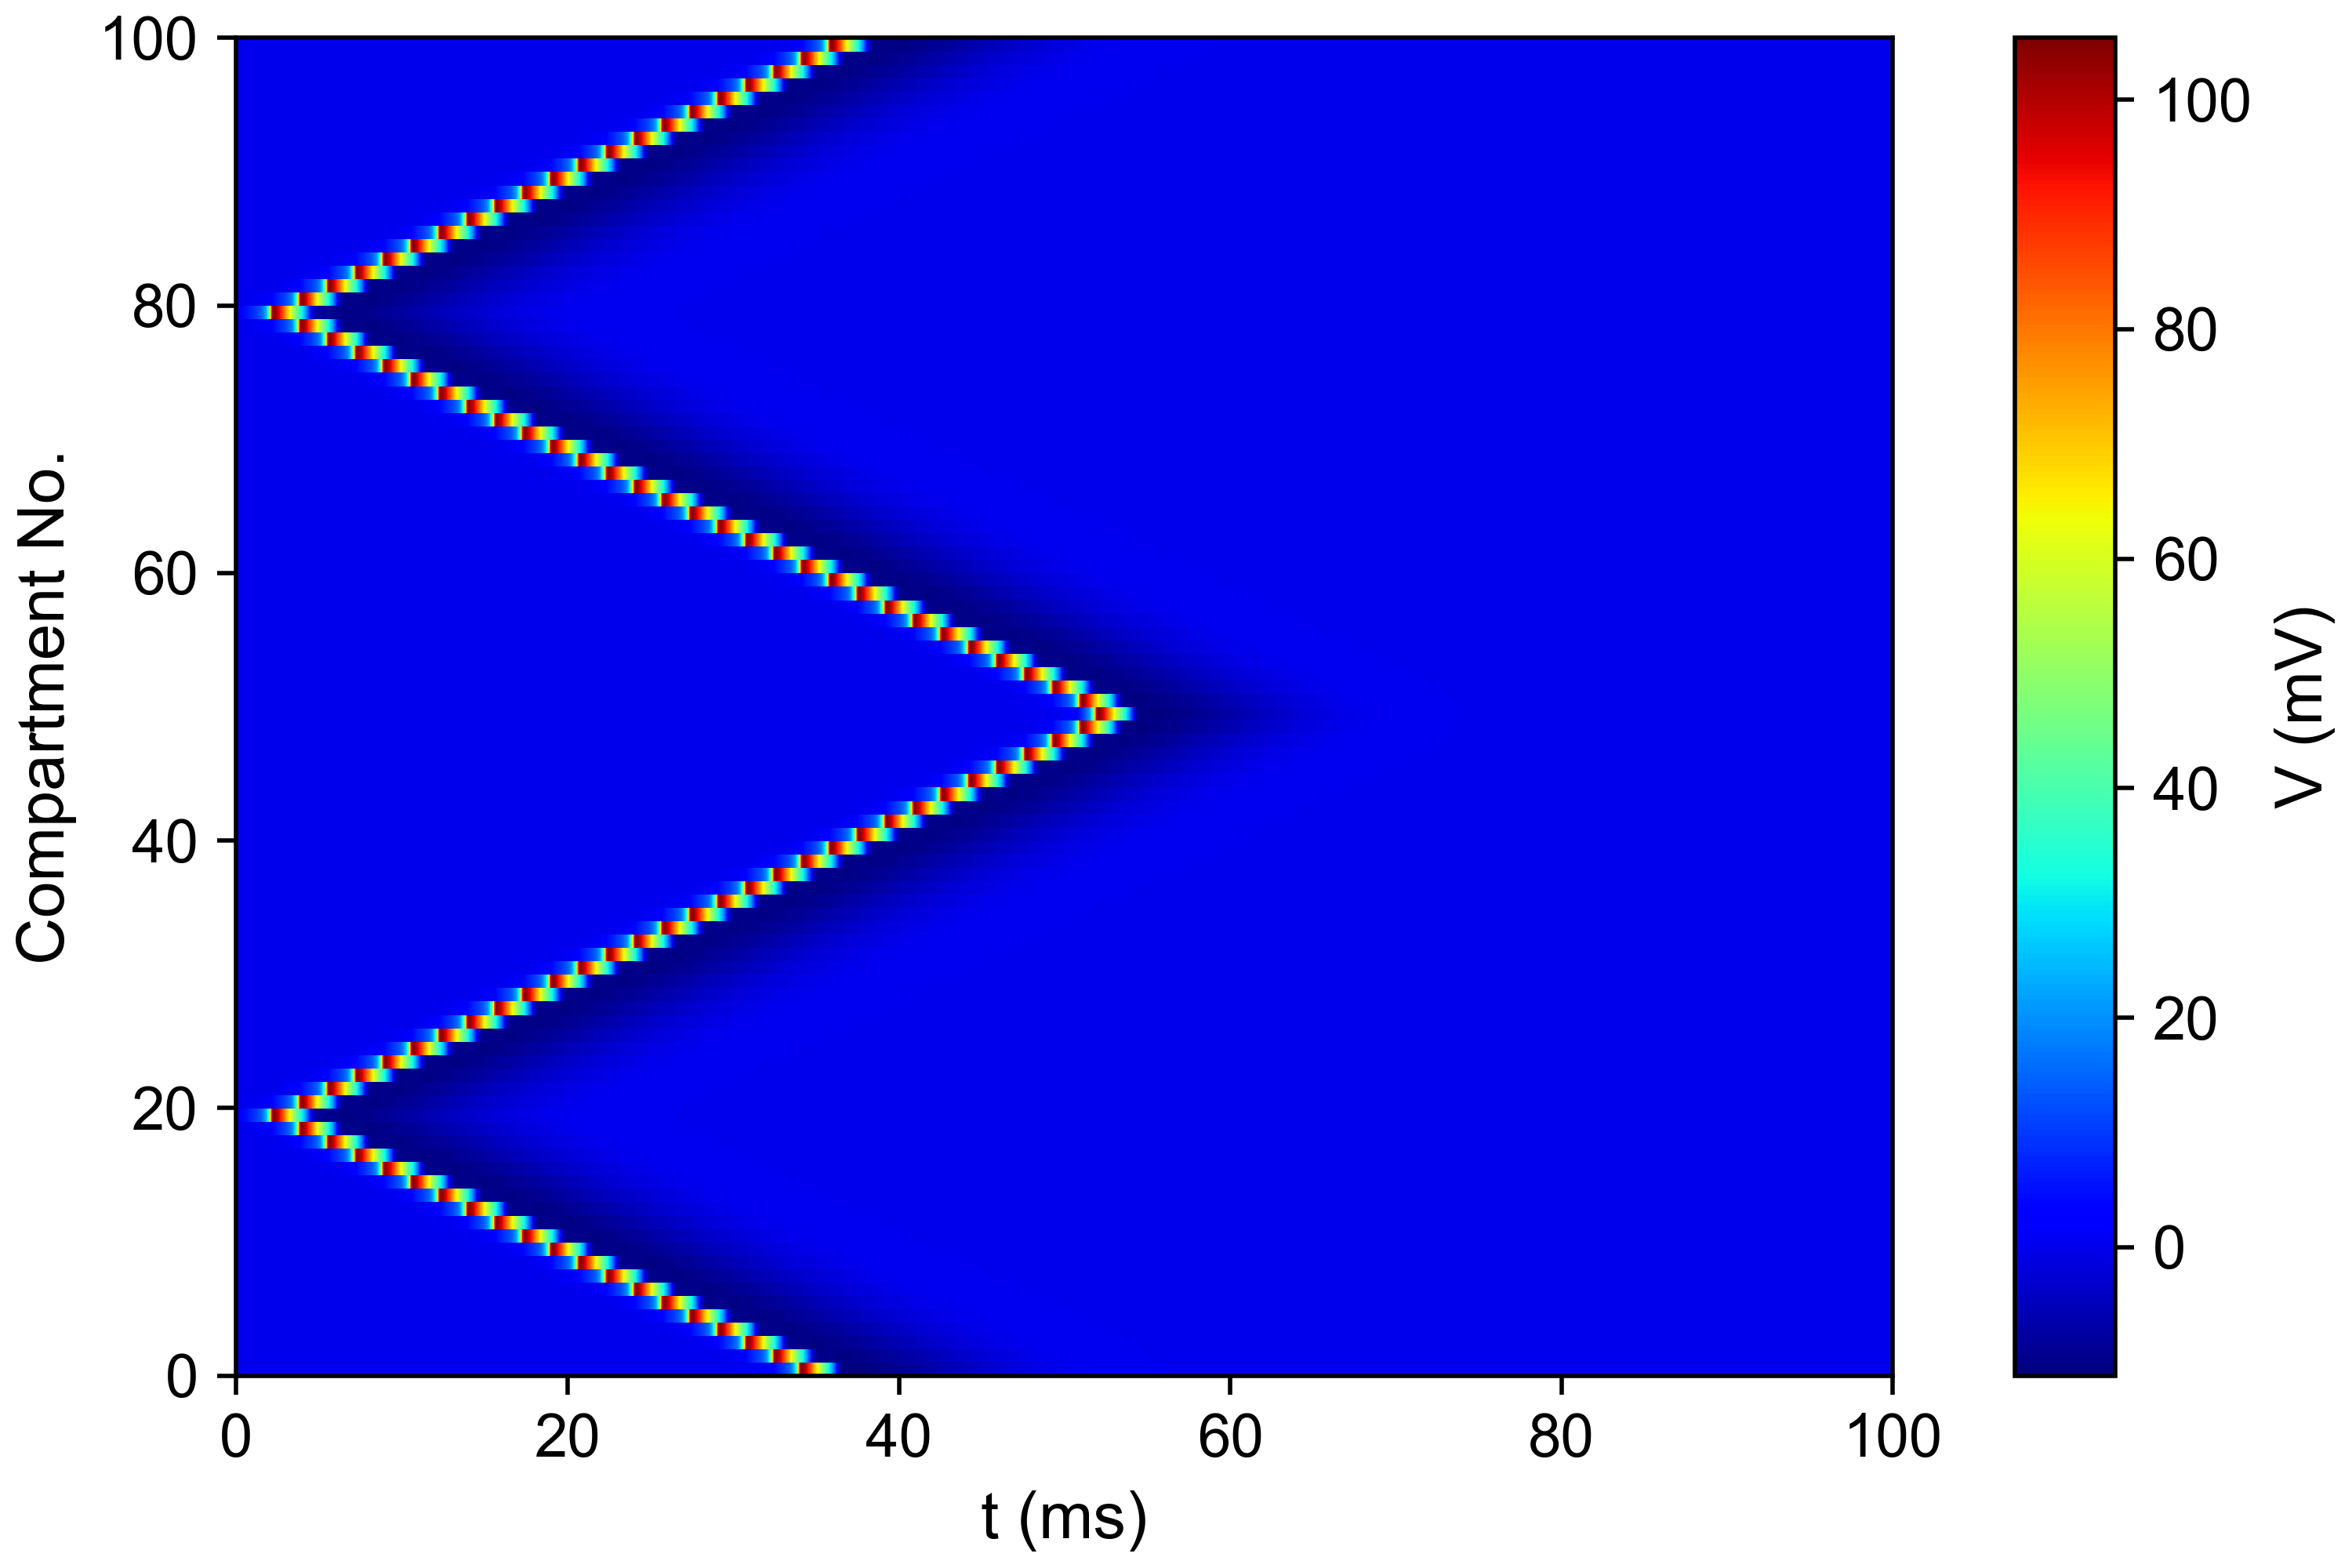
\includegraphics[width=0.9\textwidth]{figures/potential_case2.png}
	\caption{Potential for second case}
	\label{fig:2}
\end{figure}

\newpage
\section{Experiments}

The parameters of the model that can be investigated are the membrane capacitance $C_m$ and the axonal resistance $R_a$. To explore the effect of these variables only the first case from above is investigated since the underlying propagation mechanism is the same in both cases. 

Figures \ref{fig:resistance} and \ref{fig:capacitance} show the effect of increasing and decreasing the parameters with respect to the base case ($C_m=1 \mu F$, $R_a = 7.96k\Omega$). The parameters from the base case are multiplied with the scalars $s \in \{0.5, 1, 1.3, 2\}$ to produce the four plots in each figure. The parameters all control the propagation speed of the action potential. A greater slope in the plot means a higher propagation speed as more compartments are surpassed in less time. 

\textbf{Effects of Axonal Resistance}

The axonal resistance depends on three parameters as shown in equation \ref{R}. It is directly proportional to the electrical resistivity $\rho$ and the length $l$ of the myelinated axon. The resistance is inversely proportional to the cross-sectional area $A$ of the axon. 

\begin{equation}\label{R}
R_a=\rho \frac{\ell}{A}
\end{equation}

Figure \ref{fig:resistance} shows that decreasing the axonal resistance $R_a$ leads to a higher propagation speed. This can be explained with Ohm's law in equation \ref{ohm}. If the resistance decreases at a constant potential the current through the axon must increase. Hence with a higher conductance more current (i.e charges per second) can pass through the axon. Therefore the potential in the adjacent compartment can rise above the firing threshold sooner and the action potential can travel faster. Vice versa increasing the axonal resistance leads to slower signal propagation.

\begin{equation}\label{ohm}
	R = \frac{V}{I}
\end{equation}

If the axonal resistance rises above a certain threshold the action potential cannot propagate any further. This is shown in the fourth plot in figure \ref{fig:resistance}. Not enough charge can flow through the axon at once to lift the membrane potential in the adjacent cell above the firing threshold to elicit another action potential. 

\textbf{Effects of Capacitance}

Figure \ref{fig:capacitance} demonstrates that the membrane capacitance has a similar effect on the propagation speed as the axonal resistance: reducing the membrane capacitance increases propagation speed and vice versa. Capacitance is reduced by increasing the effective thickness of the membrane, which results in a bigger separation of ions between intracellular and extracellular fluid. Through smaller capacitance, less charged particles are stored on both sides of the membrane. Thus it is easier to change the membrane potential which allows sodium ions to move more freely along the axon. This results in faster conduction.

Again, it can be observed that if the membrane capacitance rises above a certain threshold the action potential can not propagate further than a few compartments. This is because the membrane capacitance is so high that the stimulating potential from the previous cell is not high enough to induce an ion flow across the membrane, which is needed to form another action potential. 

\begin{figure}[p]
	\centering
	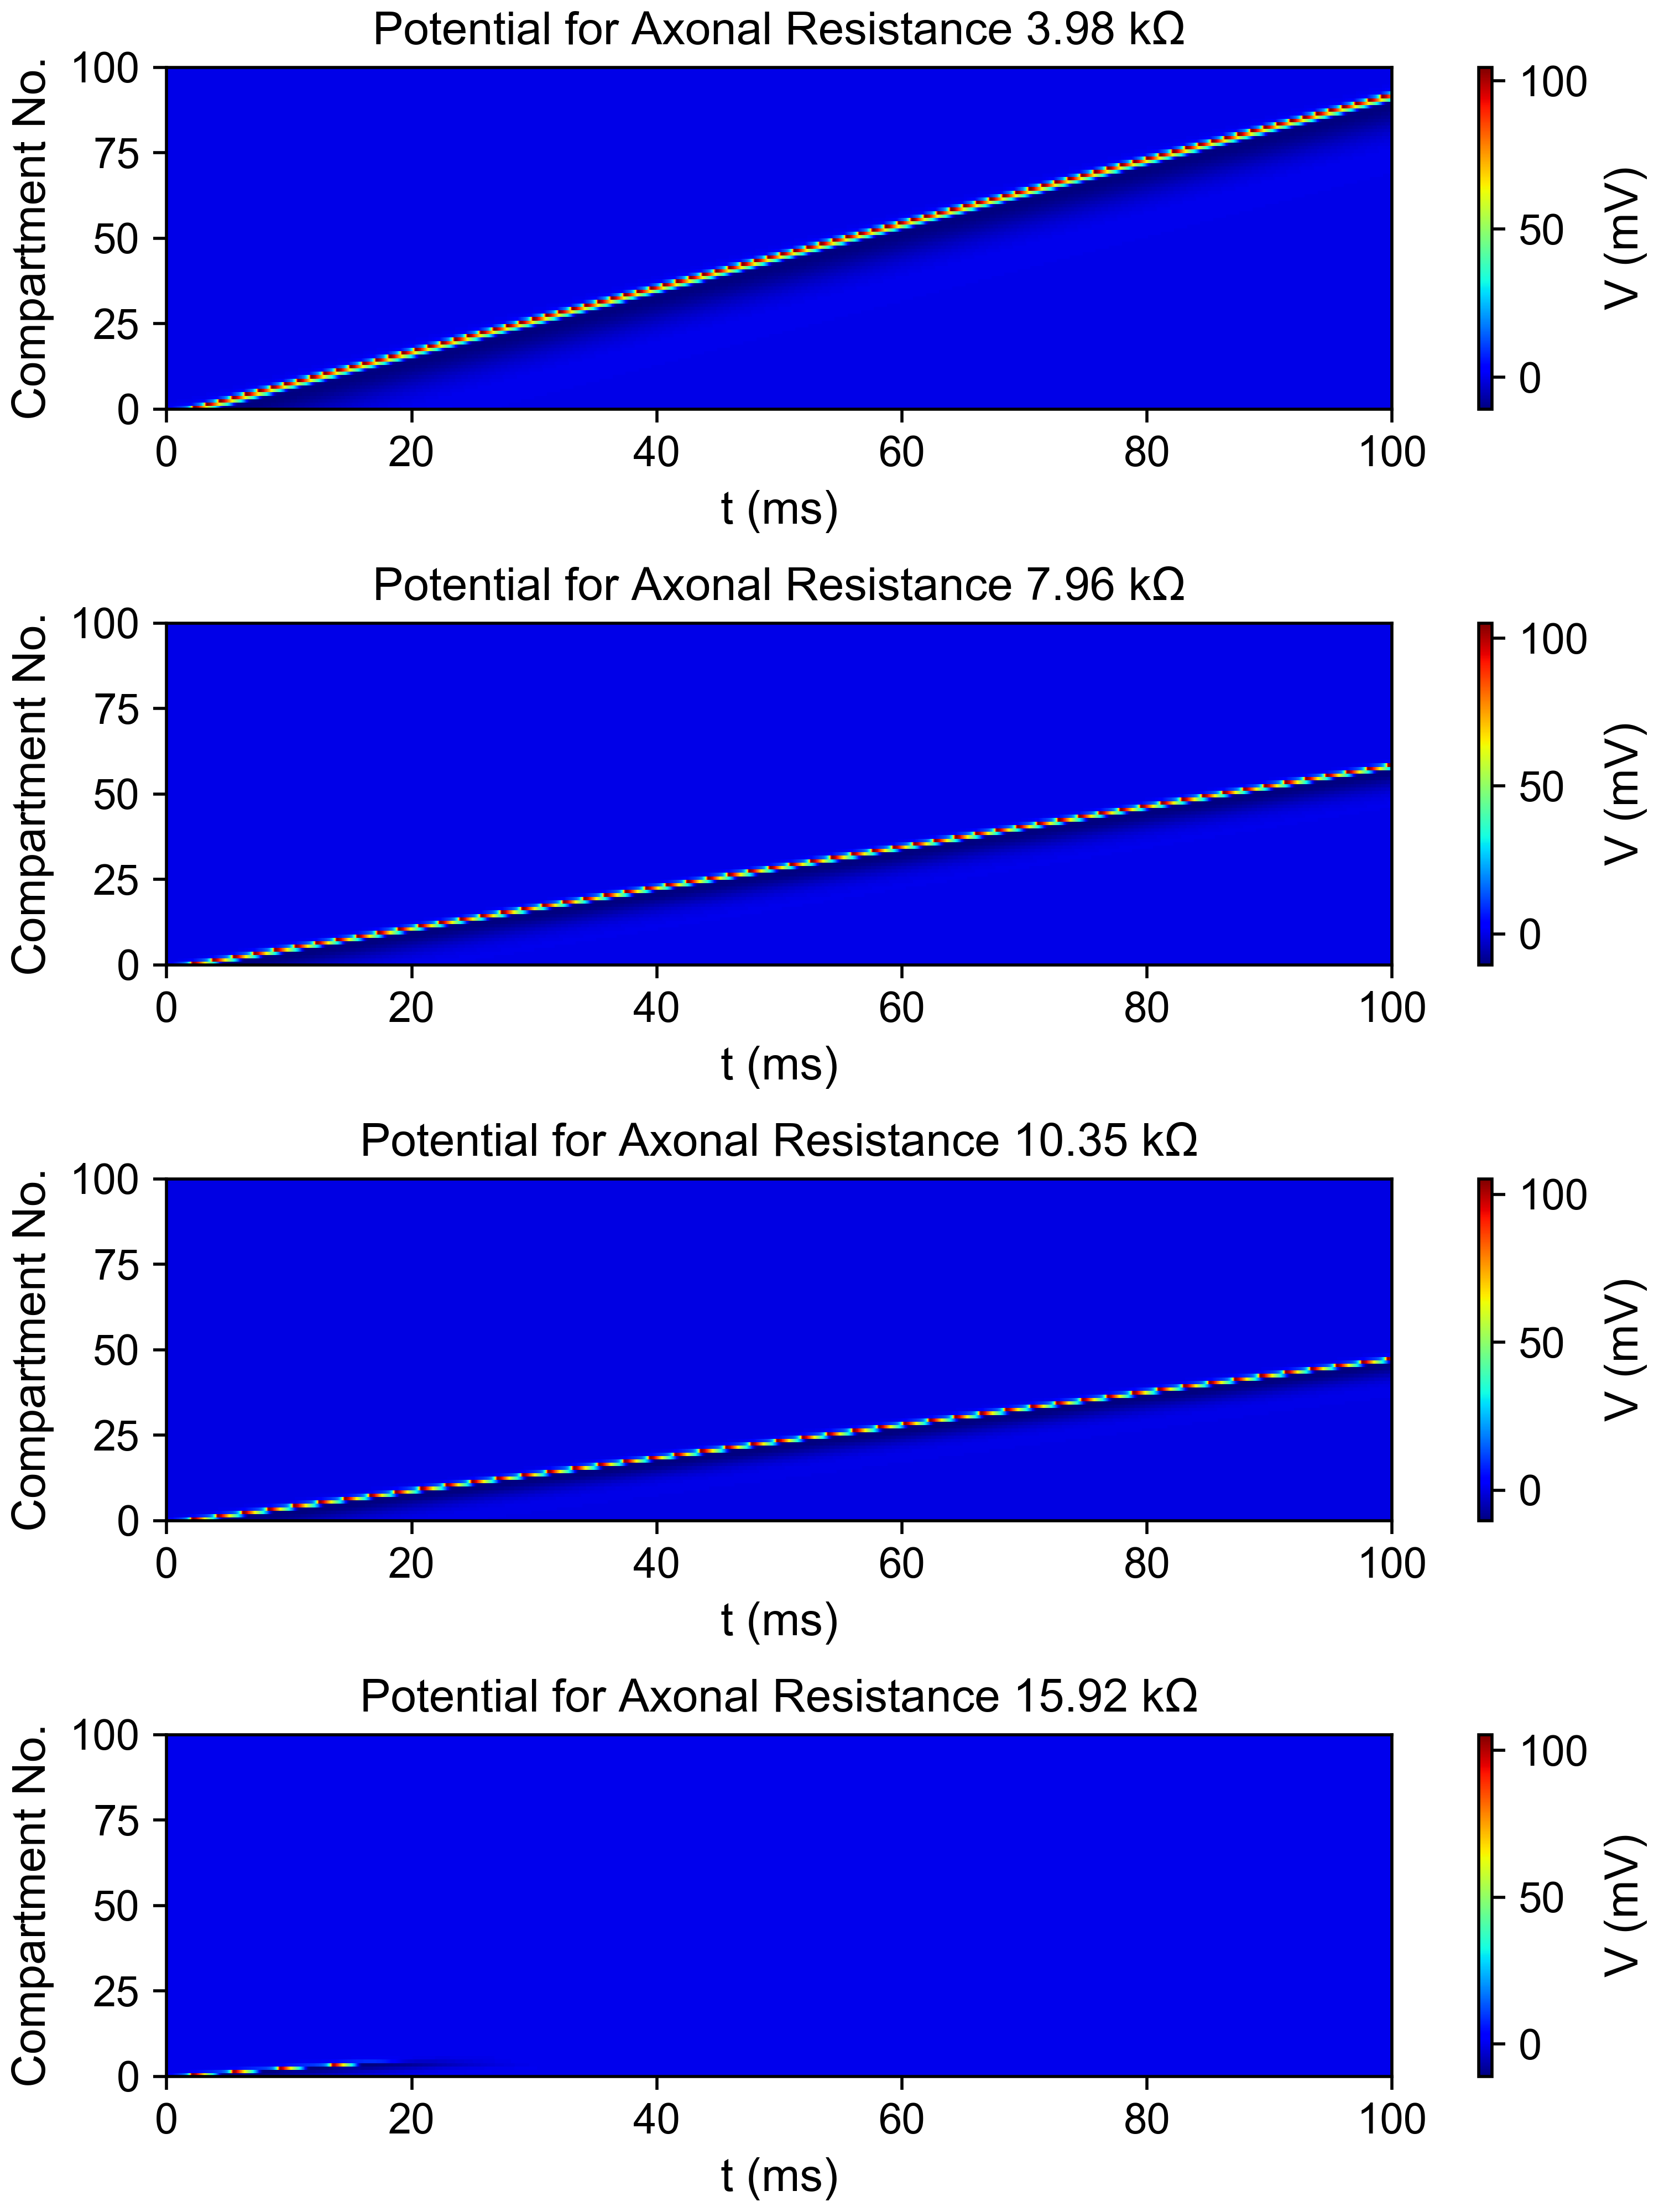
\includegraphics[width=0.9\textwidth]{figures/potential_experiments_resistance}
	\caption{Potential for different resistances}
	\label{fig:resistance}
\end{figure}
\begin{figure}[p]
	\centering
	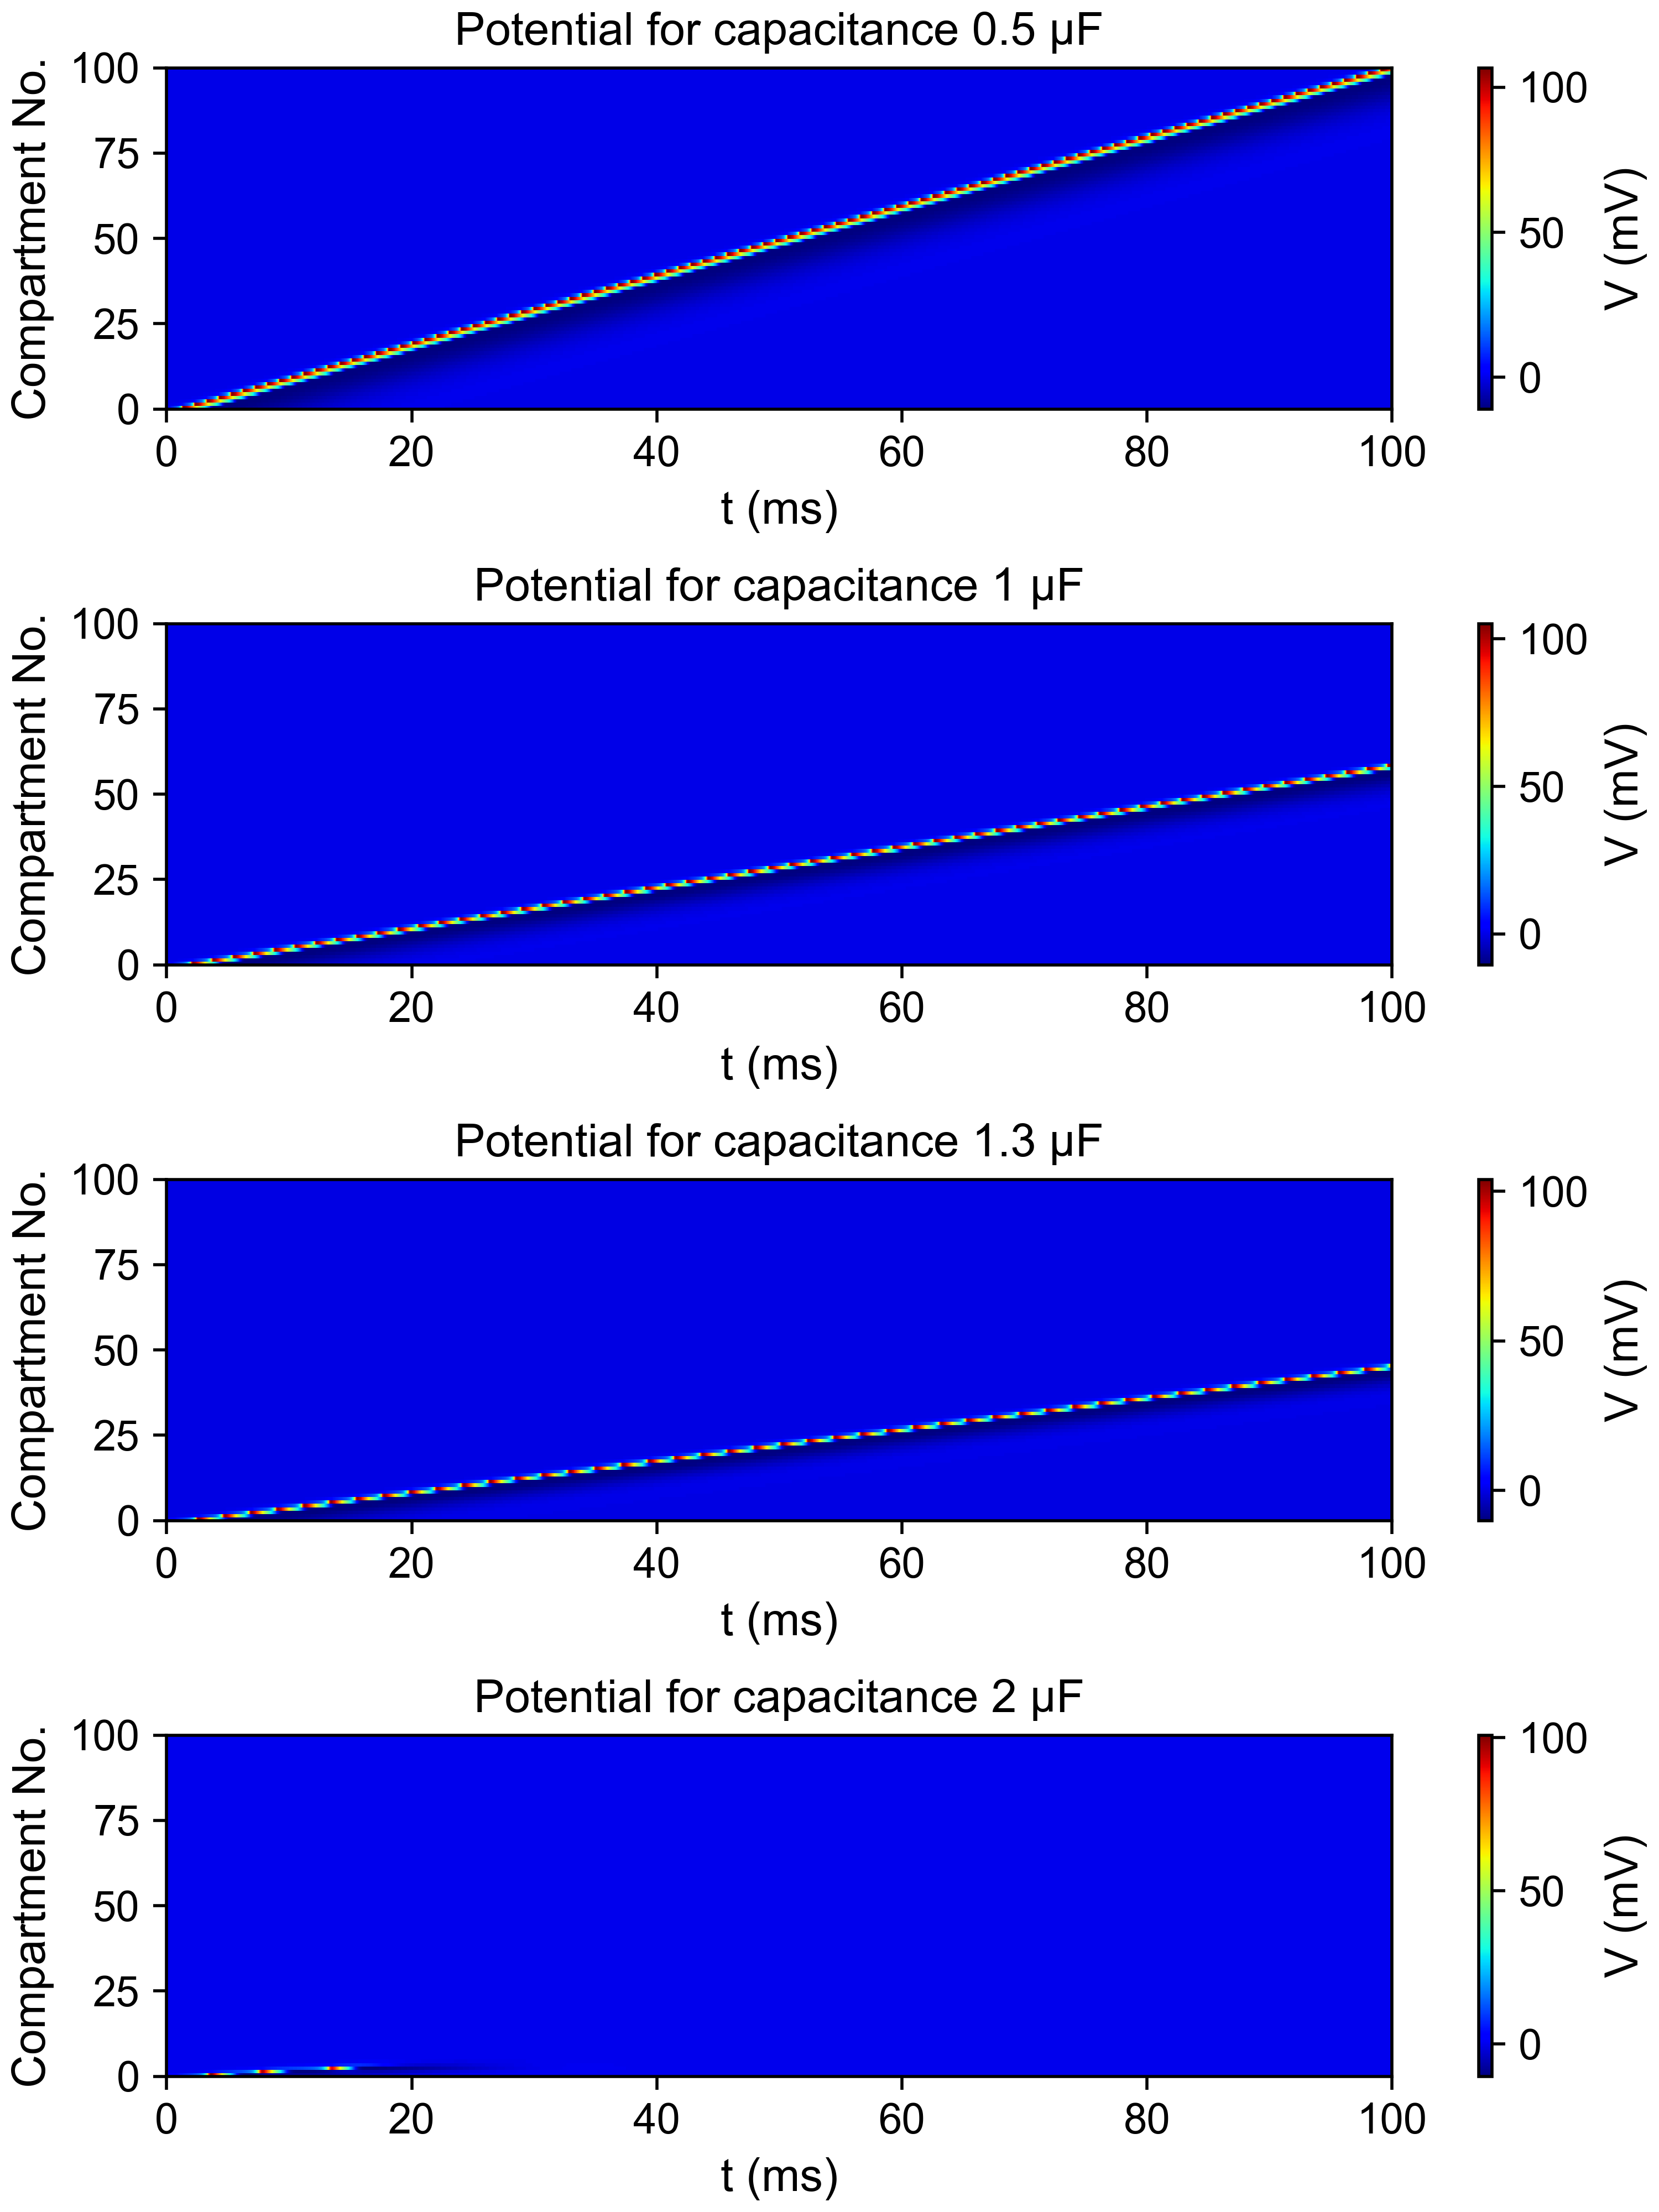
\includegraphics[width=0.9\textwidth]{figures/potential_experiments_capacitance}
	\caption{Potential for different capacities}
	\label{fig:capacitance}
\end{figure}

\end{document}